\subsection{Available requests: an expansion-bounded follow-up}
\label{sec:followup-protocol}
Flat replay knows the finished search trace. A cap on outstanding transactions limits how much it offers at once, but can still offer a later expansion before the reads that discovered it have completed. This raises a directly related question: does placement behave differently when the next work is withheld until its preceding memory work completes?

The follow-up introduces \emph{phases}. An adjacency-list payload forms one phase. The candidate vector reads that follow that list form the next. The frontend drains all reads in each phase before accepting the next phase; initial vector reads and graph-level entry reads receive separate phases. Each candidate is checked against its preceding list at the same level. Figure~\ref{fig:phases} illustrates the boundary. The existing draining query marker represents a phase ID, with a separate map back to the original query. No simulator timing rule is changed, and bank-row state remains warm.

\begin{figure}[htbp]\centering
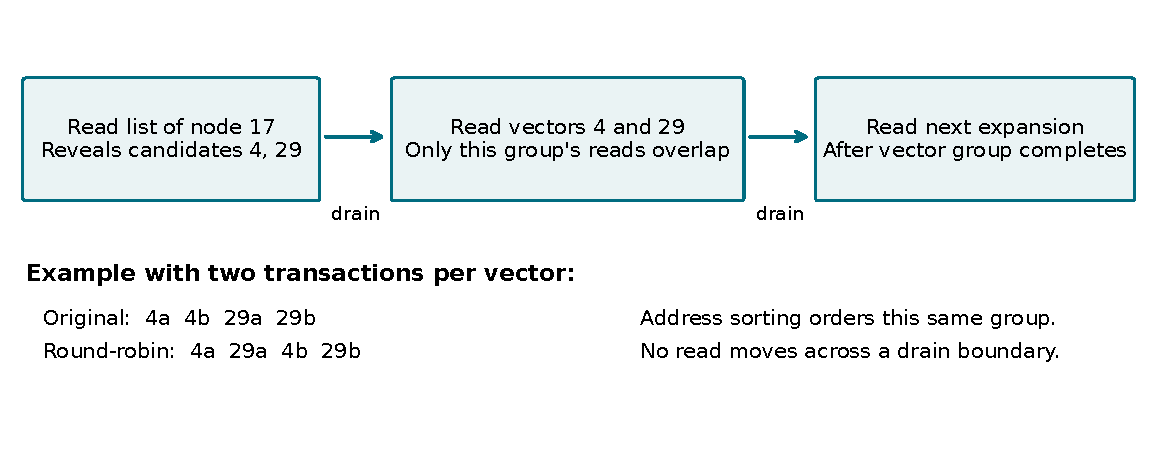
\includegraphics[width=\textwidth]{generated/followup_phases.pdf}
\caption[Requests available within an expansion]{Expansion-bounded replay and two illustrative vector chunks. Real 512-byte and 128-byte vectors contain sixteen and four transactions respectively. An arrow means that earlier reads must complete; computation is not timed.}\label{fig:phases}
\end{figure}

Inside each vector phase, the original transaction order is compared with two schedules. \emph{Address sorting} places the available transactions in ascending address order. \emph{Transaction round-robin} offers the first chunk of each vector, then the second chunk of each, and so on. Sorting aims to bring nearby addresses together; round-robin aims to expose several vectors earlier. Every transaction, including duplicates, remains in its original phase. Neither schedule borrows requests from a later expansion. Their scheduling and buffering costs are omitted, so they measure opportunities before implementation overhead.

The model assumes that the selected candidate vectors within an expansion can be fetched together. It does not implement the search's distance arithmetic or instruction-level control flow, and can expose more intra-expansion overlap than stock execution. Conversely, draining every expansion excludes overlap that a more asynchronous implementation might achieve. It is a defined memory-dependency sensitivity, not a cycle-exact PIM engine or a bound on every implementation.

The fixed design adds 494 replays: 19 graph/split pairs, two footprints, and 13 conditions per pair/footprint. The conditions comprise three published layouts under flat replay; identity, BFS, query-aware and the three published layouts under expansion boundaries; and both alternative schedules on BFS and query-aware placement. The 19 pairs are the ten reference splits plus three splits for each additional construction. The default mapper, open-page controller and 64-transaction limit are unchanged. The original 791 results remain available. The design was recorded before follow-up timings, with no method removed after observing its result. Because the queries were used previously, these are exploratory extensions rather than an independent validation set.

For a bounded query, service begins at the first arrival in its first phase and ends at the last departure in its final phase. Thus the reported interval includes the gaps between phases. Raw phase means are not reported as query means. Placement comparisons match both boundary mode and baseline; schedule comparisons use the same layout with original-order bounded replay. Ten-split intervals remain conditional on the reference graph. Additional constructions are reported separately on matched splits one through three. All layouts are compared with identity and BFS in the retained summaries.
